\subsection{Functional Role}

Before analyzing in detail the functional role covered by the java class assigned us for code inspection, a brief description of the context and explanation of the most relevant elements is provided.  

\subsubsection{OFBIz overview}
The Open For Business project is an enterprise-oriented suite of applications developed to support most of the aspects that an enterprise application has to take care of.

The applications share the same underlying architecture, using common data, logic and process components.

A loosely coupled approach is used as base for the architecture, allowing an easy extension of the suite itself.

Each application is loosely coupled with the others, easing the updating and the extension.

\subsubsection{Entities and Services}
As stated by the official documentation:

\begin{itemize}
	\item \textbf{Entities}: an entity is a relational data construct that contains any number of Fields and can be related to other entities. Basic entities correspond to actual database structures.
	\item \textbf{Services}: a service is a simple process that performs a specific operation.
\end{itemize}

\subsubsection{Project's architecture}

The architecture of the entire suite is composed by 4 sets of components:

\begin{itemize}
	\item \textbf{Framework}
	\item \textbf{Applications}
	\item \textbf{Special Purpose}
	\item \textbf{Hot-deploy}
\end{itemize}

The sets of components, as well the contained components, are in a dependency relationship according to the dependency-arcs shown in the following diagram.

The dependency flow goes from top to bottom, either for component sets and for components.

This means that components and applications on the top are dependent on elements on the bottom of the same diagram. The viceversa should not be allowed.

The type of dependency may vary: foreign key dependency in the data model, application's service calling another application's service and so forth.

\begin{figure}[H]
	\centerline{
		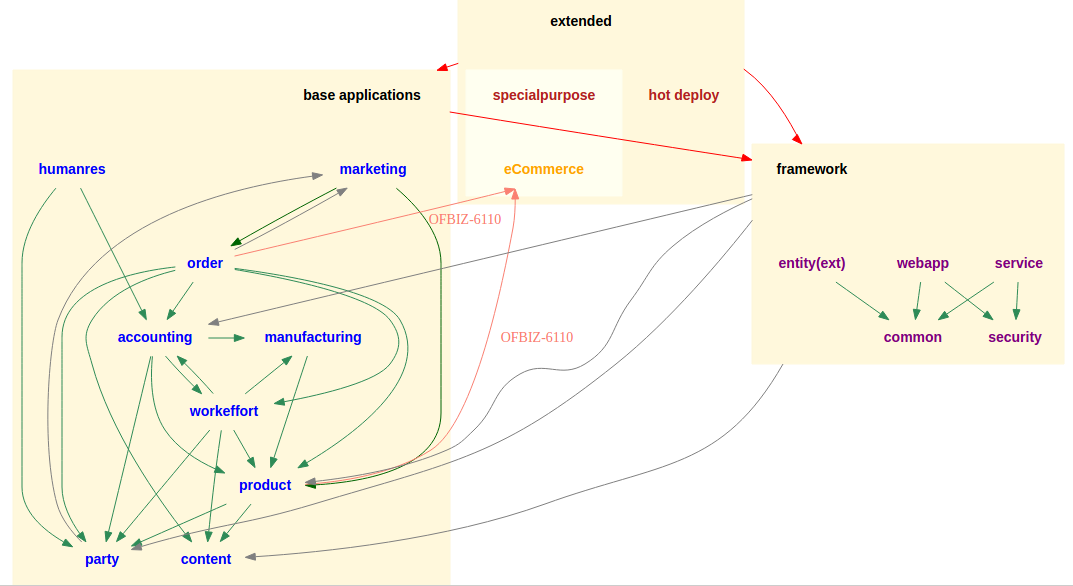
\includegraphics[width=350px]{../Datas/images/dependencies.png}
	}
	\label{fig:components-dependencies}
	\caption{Components dependencies}
\end{figure}

As can be seen, there's a relation of dependency between the human resource application and the party application.
\newpage

\subsubsection{Parties}
According to the {\textit{OFBIz project's overview}}\footnote{https://cwiki.apache.org/confluence/display/OFBIZ/Component+and+Component+Set+Dependencies}:

\textit{Party can be either a Person, or a group of Parties. A Party Group could be a company, an organization within the company, a supplier, a customer, and so forth.
Information that describes Parties or is directly related to Parties is contained in these entities.}

According to the party's data model, each party, either a person, a group and so forth, is identified by a unique ID number.

\subsubsection{Human Resource Entities}

According to the \textit{OFBIz project overview}:

\textit{The Human Resources entities are used to keep track of positions, responsibilities, skills, employment, termination, benefits, training, pay grades and payroll preferences, performance reviews, resumes and applications, and other Human Resources related information.}

\subsubsection{Employee Position}

Also abbreviated as \textit{position}, it is an entity used to represent a work position inside the company.
Quoting the \textit{official documentation of the project}\footnote{https://cwiki.apache.org/confluence/display/OFBIZ/Employee+Position}:

\textit{In OFBiz a position is the authorization, typically from the budget of an internal organization, for the Company to engage one person to do a job. OFBiz handles positions in a flexible manner so you can think of a position as an authorization for a full-time equivalent (FTE).}

\textit{This means that you can fulfill a position with a person in a number of different ways. You can fill a position with one full time person, change the assignment of a position from one person to another over time, or split a position across more then one person at the same a time.}

\textit{As implemented a position can be fulfilled by \textbf{either a person or organization}.}

The data model\footnote{https://cwiki.apache.org/confluence/display/OFBIZ/Data+Model+Diagrams} representing a employee position is quite huge and complex, so only the essential part for our analysis are shown and described.

\textbf{NB:}\textit{The whole data model diagram on the wiki is not up to date, therefore there could be some discrepancy between it and the documentation.}

\begin{figure}[H]
	\centerline{
		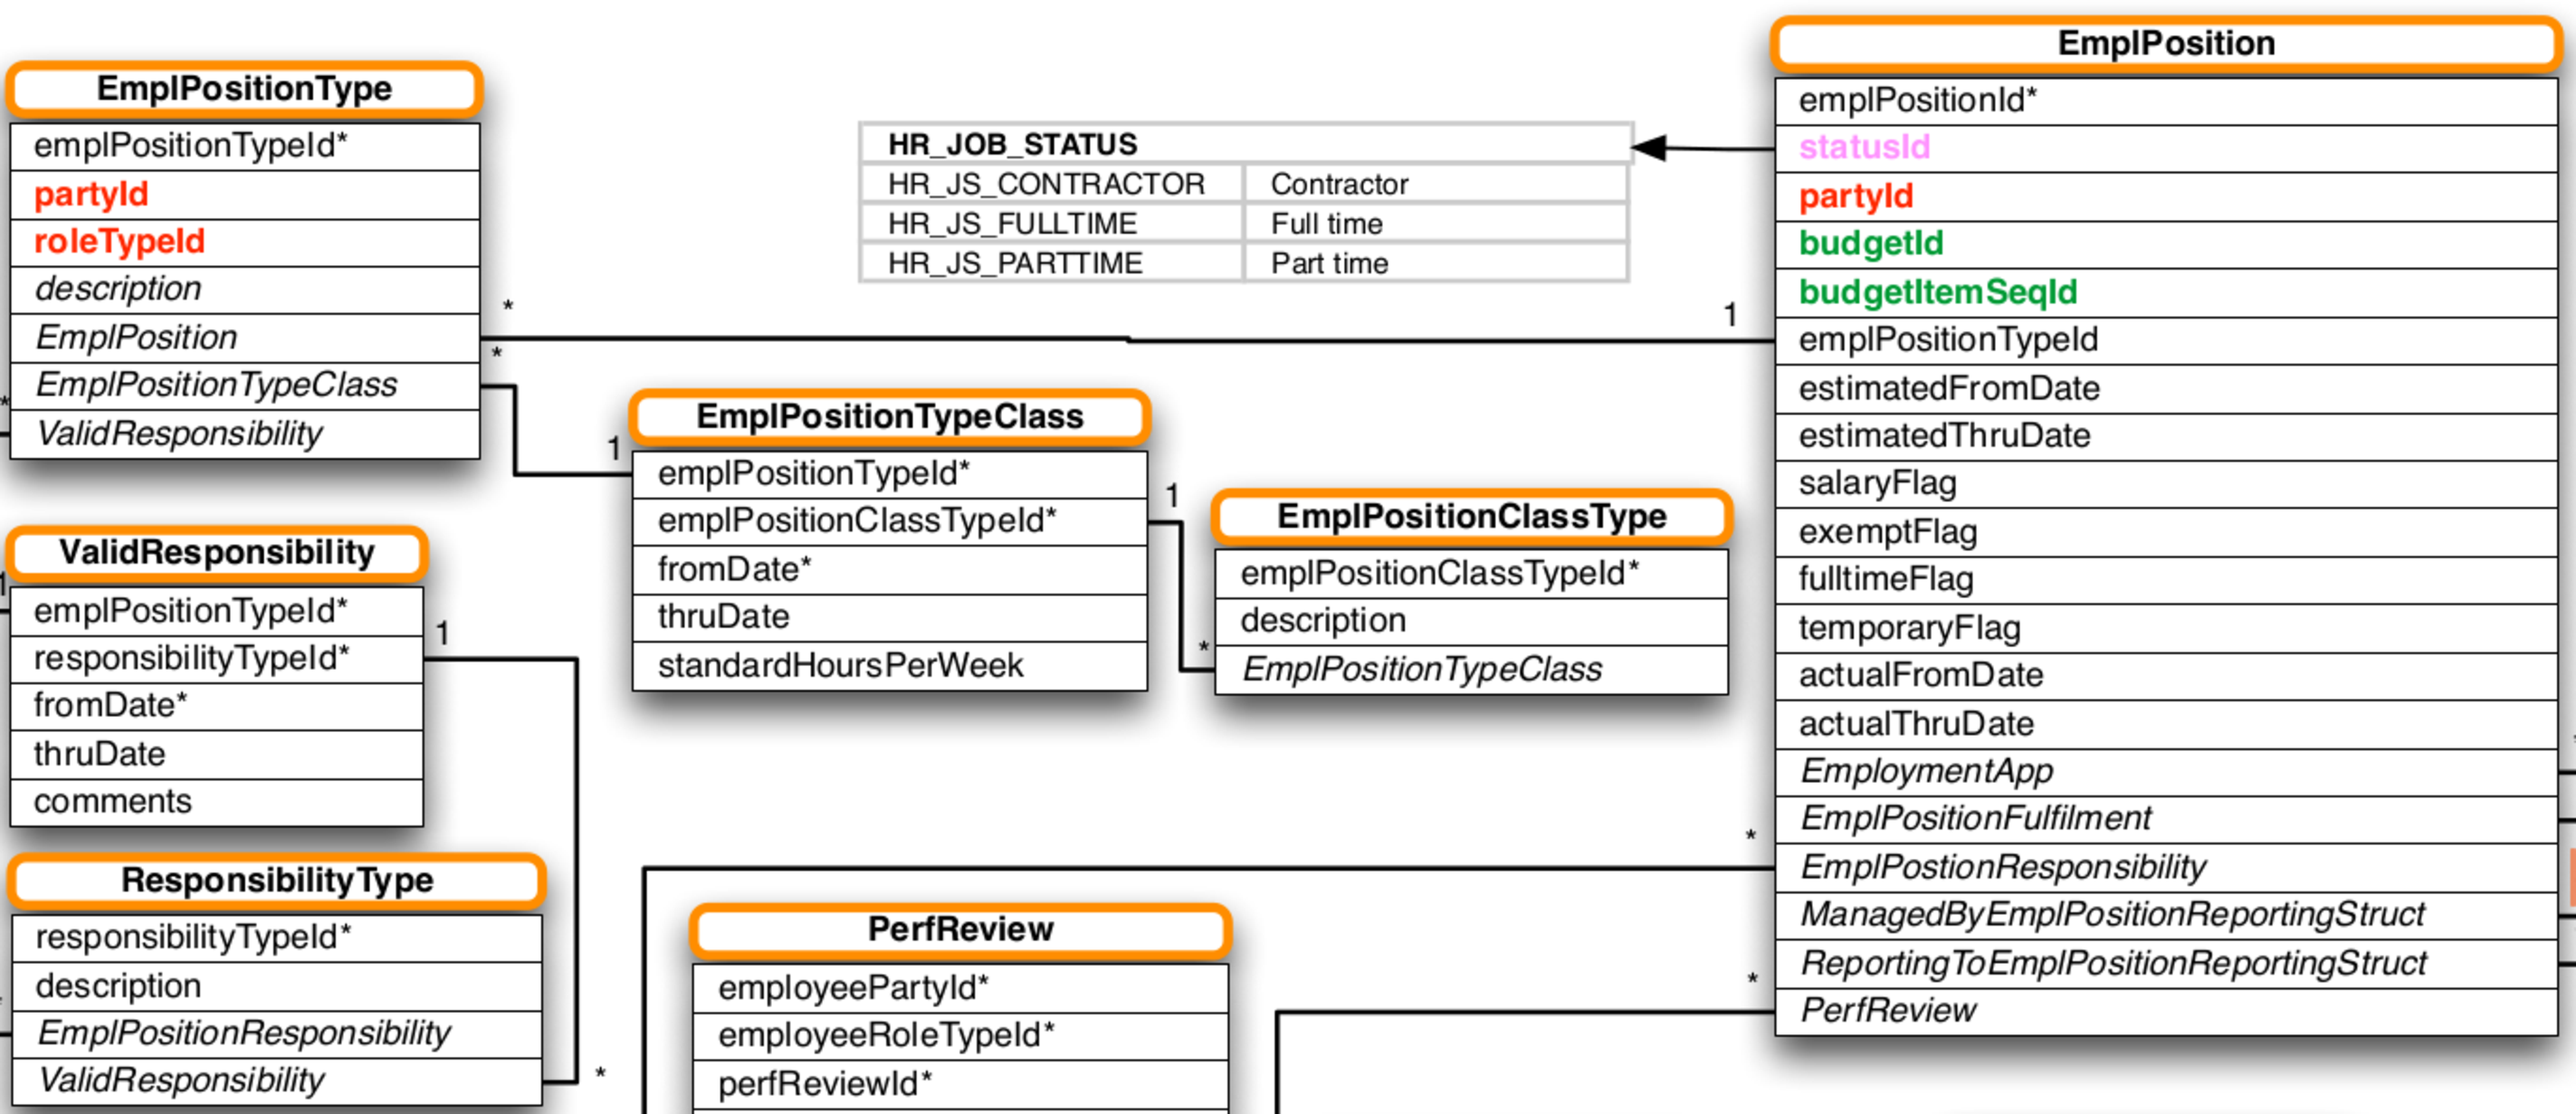
\includegraphics[width=350px]{../Datas/images/emplPos-posType.pdf}
	}
	\label{fig:emplPos-type}
	\caption{Employ Position - Employ Position Type relationship}
\end{figure}

\begin{itemize}
	\item \textbf{EmplPosition}: entity used to represent an employee position inside the Human Resource Application. 

	Each entity is characterized by several. The most relevant for our analysis are:


	\begin{itemize}
		\item \textbf{emplPositionId:} an \textbf{unique} identifier used to distinguish a position from another one.
		\item \textbf{statusId:} a string identifying the status of the position.

		Actually, the documentation and the data model of the emplPosition entity diverge about the content of this field. 

		The former specifies that it is used to state if the position is \textbf{Active/Open}, \textbf{Inactive/Closed} or \textbf{Planned for}, while the data model diagram report is as a field specifying the type of position: \textbf{full time}, \textbf{part time} or \textbf{contractor}.

		As stated previously, the data model is not updated, therefore we take as reference what described by the documentation.
		\item \textbf{partyId}: the ID of the \textbf{Internal Organization} authorized to fill the position.
	\end{itemize}

	\item \textbf{EmplPositionType:} entity representing a possible type for a position. An example of position type is the Business Analyst or the System Administrator.
	Relevat fields are:

	\begin{itemize}
		\item \textbf{emplPositionTypeId:} unique identifier used to discern between position types.
		\item \textbf{partyId:}
		\item \textbf{description:} a description of the type of position.
		\item \textbf{EmplPosition:} identifier of the employee position having this specific type. 
	\end{itemize}  
\end{itemize}

\begin{figure}[H]
	\centerline{
		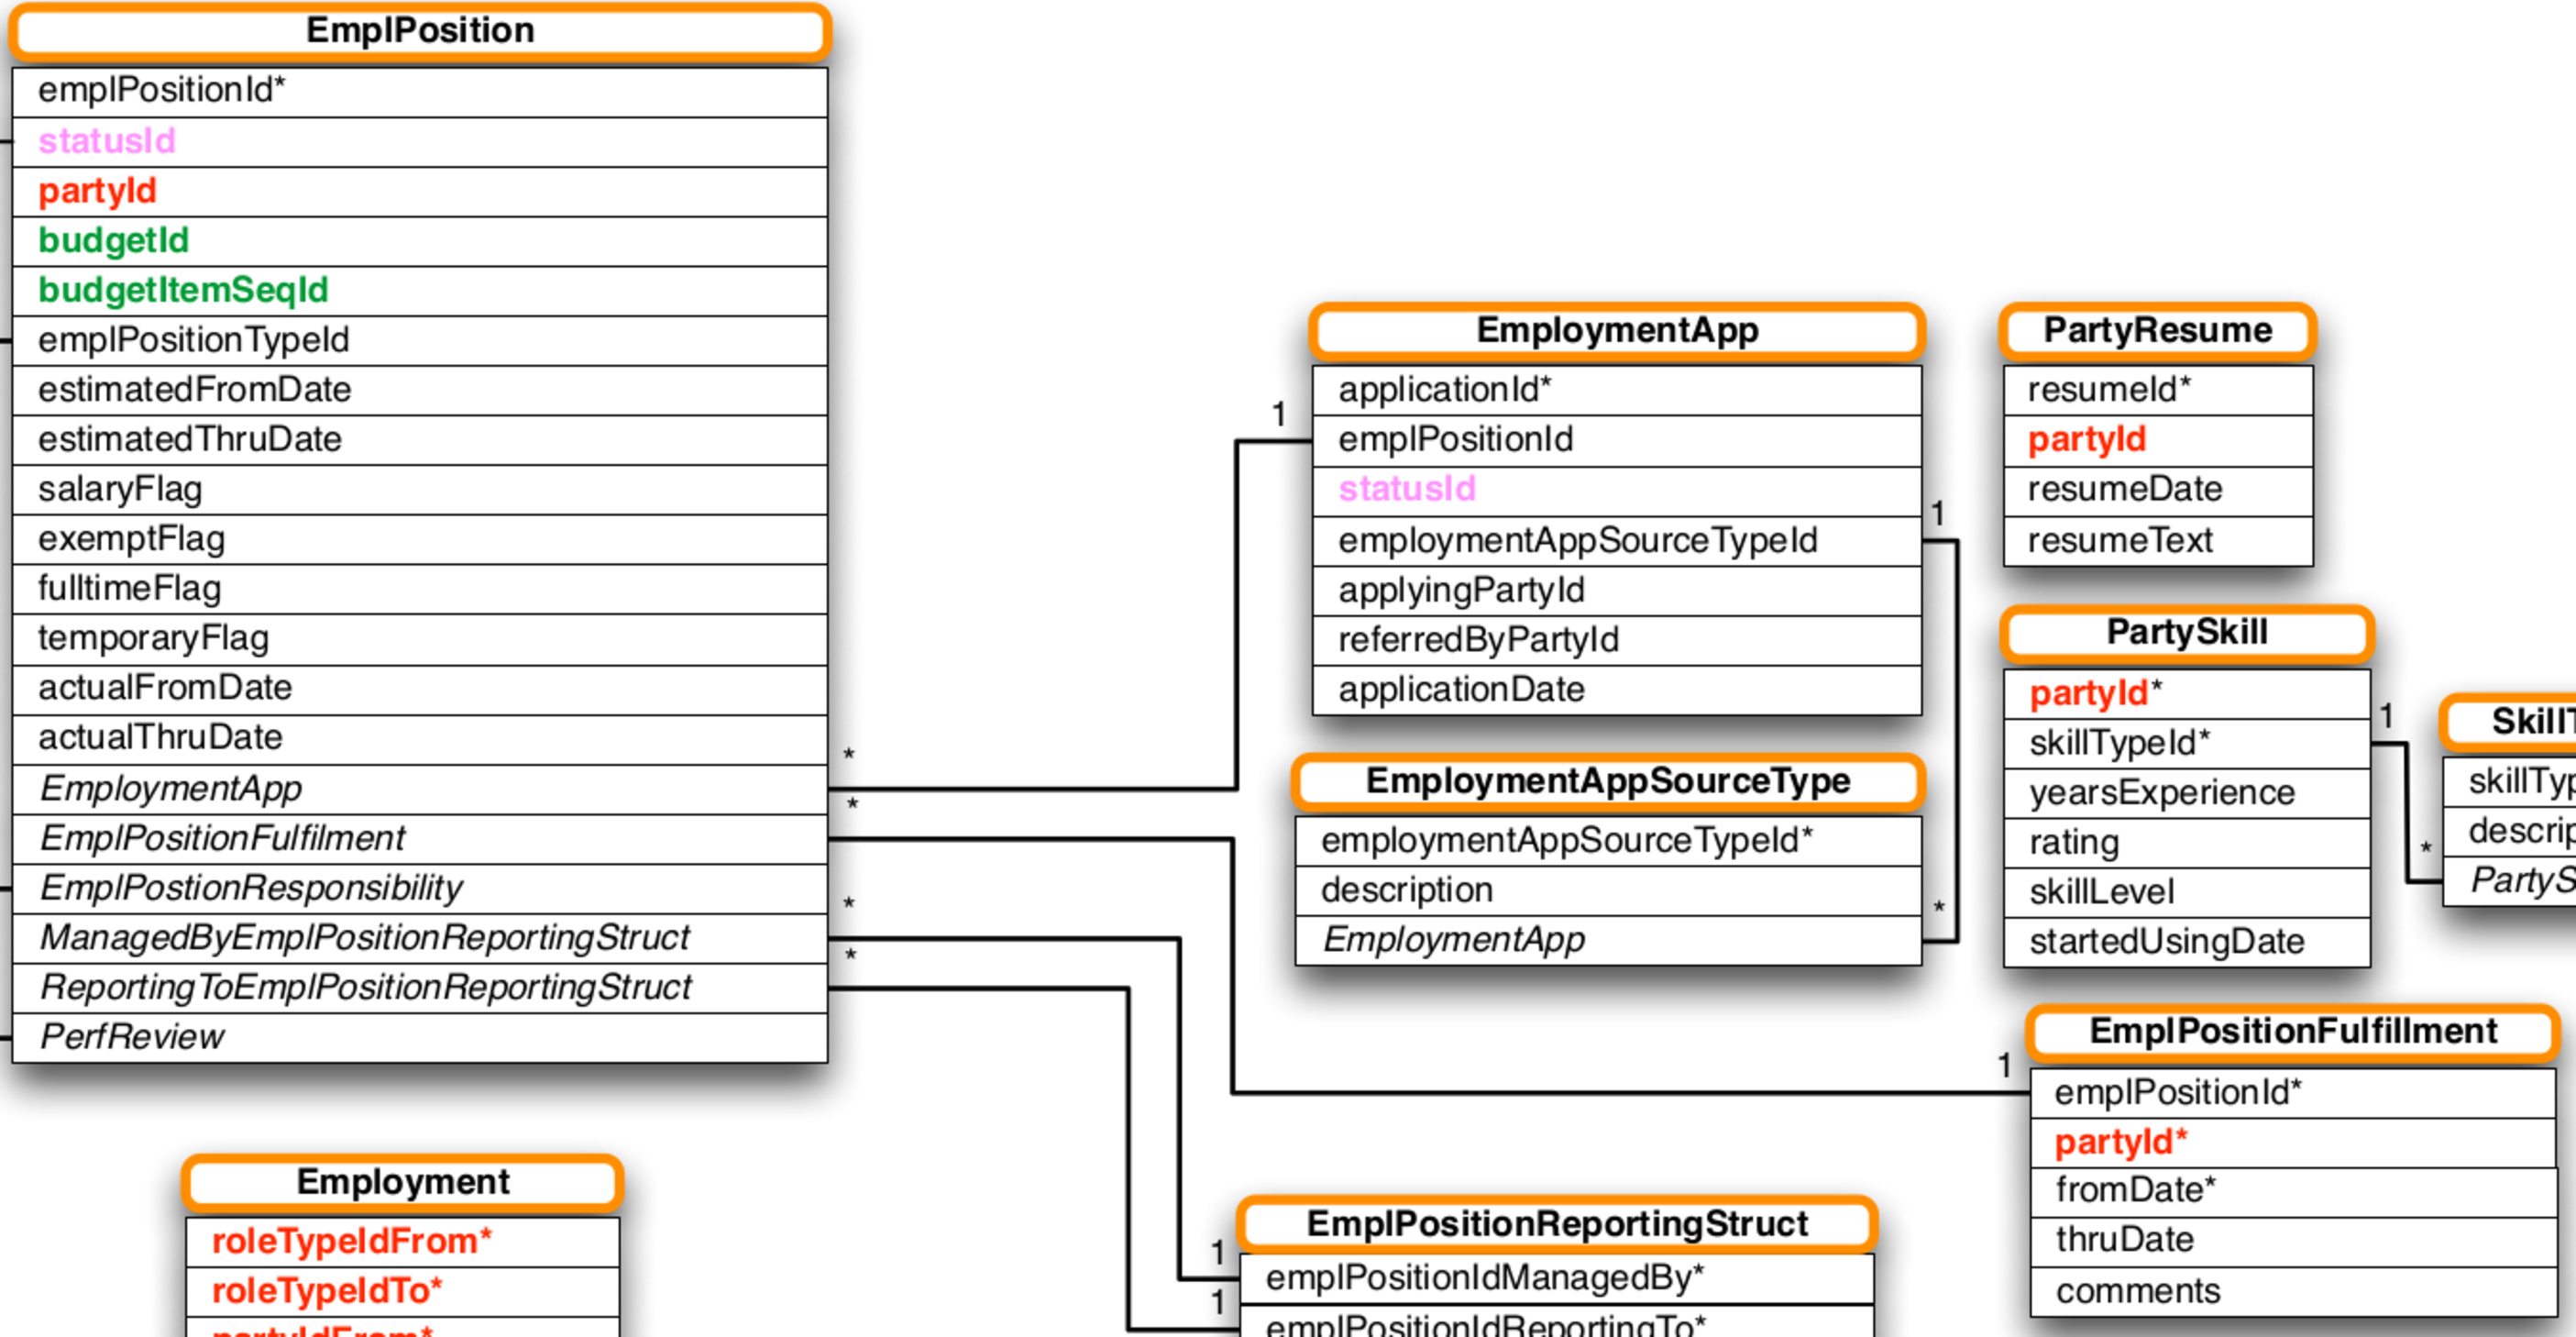
\includegraphics[width=350px]{../Datas/images/emplPos-fill.pdf}
	}
	\label{fig:emplPos-fill}
	\caption{Employee Position - Employee Position Fulfillment relationship}
\end{figure}

\begin{itemize}
	\item \textbf{EmplPositionFulfillment}: entity used to represent the party or parties that fulfill a specific position.
	Relevant informations of this entity are:

		\begin{itemize}
			\item \textbf{emplPositionId:} the ID of the position fulfilled by the party.
			\item \textbf{PartyId:} the ID of the party fulfilling the position.
			\item \textbf{fromDate:} the date from which the position is fulfilled.
		\end{itemize}
\end{itemize}

\subsubsection{Internal Organization}
Quoting the \textit{human resource glossary}\footnote{https://cwiki.apache.org/confluence/display/OFBIZ/Human+Resources+Glossary}:

\textit{Internal organization is the name of a relationship between a party group and your company.}

\textit{This relationship is used to filter party groups as being part of your company to distinguish them from other groups which are external.}

\textit{For example your marketing department is an internal organization while a suppliers sales department is not.}

\subsubsection{Human resource application:}

The human resource application comes with a predefined set of functionalities that can be used to perform HR tasks or to provide a support for the creation of more complex HR applications.\footnote{https://cwiki.apache.org/confluence/display/OFBIZ/Human+Resources+Guide} 

According to the documentation of the human Resources application\footnote{https://cwiki.apache.org/confluence/display/OFBIZ/Human+Resources+-+Main+Window}:

\textit{The Main window is the entry point into the Human Resources Application and displays the Company tree view for navigating to the main menu items.}

\textit{There are three node types in the tree, each identified by a different icon. The top of the tree represents your Company, the highest level in the organization. The Company and departments under the Company can have sub departments or positions. Under positions are the people who fulfill the position.}

Furthermore, as stated by the documentation, from the main screen of the application is possible:

\begin{itemize}
	\item Navigate the company hierarchy, viewing departements, position and people.
	\item Add or remove a department
	\item Add a person
	\item Quickly open the profile of any item in the tree
	\item If an item is a position, you can add a person to fulfill the position.
\end{itemize}

\paragraph{The HumanResEvents class}:

Despite the misleading namename given to this class, the main purpose of this class is to support the building of the company tree, 
% 7h:30min
This class is supposed to support all the functionalities that the humanres application backbone has to provide. This has been already listed in the previous paragraph.

Up to these release, the class presents 4 methods: one public and the rest private.
The private methods are used as helper functions by the public one.

In the following the methods composing the class are described in details.

\paragraph{getChildHRCategoryTree:}

Only public method exposed by the HumanResEvents class. It's functional role is to manage the request of visualization of a given node of the tree describing the enterprise hierarchy.

The method retrieves the informations regarding the child requested. This, according to the party definition, may be an employee or the company or a department (partyGroup).

If the former is the case, the informations of the employee selected are returned. If the latter is the case, the departments that are child of the department selected or of the company, in the case the root of the tree has been selected, are returned, along with the informations about the employees that work in the selected department or company

% This can be infered both from the informations in the xml files presented before and the few comments in the method.


\paragraph{getCurrentEmployeeDetails:}

Helper method used to retrieve the informations of an employee that currently is covering a specific position.
The position is identified by the "partyID" parameter.
First retrieve the presence of a position matching the ID passed as parameter.
Then, retrieves the list of employment fulfillments regarding that position. Indeed, more than an employee can cover that position at the same time.
The filter returns only the current fulfillment.
The query count is used, but the interval is [0, 1].

% A position can be fulfilled at the same time by different persons!
% https://cwiki.apache.org/confluence/display/OFBIZ/Employee+Position
% As reported by the documentation (link line above), the position
% may be fulfilled either by a person or an organization.
% NB: the person is not necessary an employee of out company.
% People may be employees of your Company, a company you do business with, or unaffiliated contract employees

For each fulfillment, the employee name and surname is retrieved.
Maybe the fulfillment is covered by a company or organization.
The informations retrieved are the Name and Surnamen of the employee.


% l.107: maybe this is done by l.101
% l.264: EMPL_POS_INACTIVE is a status code not reported in the official documentation
